% homework
% 20161121
% by hiaoxui

\documentclass[a4paper, 12pt, notitlepage]{article}

\usepackage{CJKutf8}
\usepackage{indentfirst}
\usepackage{amsmath}
\usepackage{listings}
\usepackage{longtable}
\usepackage{graphicx}
\usepackage{float}

\setlength{\parindent}{2em} 

\begin{CJK*}{UTF8}{gbsn}
\begin{document}

\title{第六次OS作业}
\author{秦光辉\ 1500011398}
\maketitle

	\textbf{对于目录文件而言,假设一个物理块放10个目录项,一个目录下最多放40个文件;并且,下级文件是目录文件,则上级目录项指向该目录文件的首地址;如果下级文件
是普通文件,则上级目录项指向该文件的文件控制块。假设索引表放在FCB中,采用UNIX的三级索引结构。}

	\textbf{问:下图的目录结构中,如果要读取K的第一块或最后一块,需要访问硬盘最少几次,最多几次?}

\begin{figure}[h]
\centering
	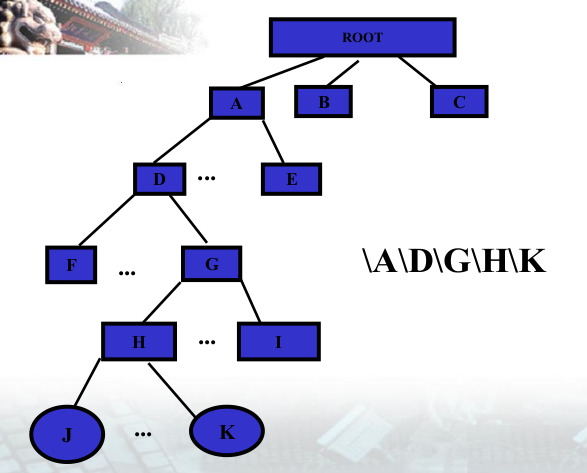
\includegraphics[scale=0.4]{hw6_figure.png}
	\caption{题图}
\end{figure}

	首先找文件的FCB. 最好的情况下, D的首地址在A的前十个块中, G在D的前十个块中, H在G的前十个块中, K在H的前十个块中. 这样我们只需要5次访问硬盘就可以找到K的FCB. \\
	
	最坏的情况下, 上述每个指针都在上一级目录的三级索引列表中才能找到. A是root的第一项, 只需要访问一次就可以找到, 其余各项都需要访问4次, 这样一共访问了硬盘17次. \\
	
	如果寻找K的第一块, 则只需要再访问一次硬盘即可, 无所谓最好与最坏. \\
	
	如果寻找K的最后一块, 这块可能位于前十个块中, 可能位于三级索引列表中. 最好的情况下只需要访问一次, 最坏的情况下需要访问4次. \\
	
	综上所述, 我们可以得到如下结论:
	
\begin{center}
	\begin{longtable}{|c|c|c|c|c|c|}
	
	\hline
	 & 寻找K的第一块 & 寻找K的最后一块 \\
	\hline
	最好 & 6 & 6 \\
	\hline
	最坏 & 18 & 21 \\
	\hline
	
	\end{longtable}
\end{center}

\end{CJK*}
\end{document}